\documentclass[a4paper]{article}

\usepackage[english]{babel}
\usepackage[utf8]{inputenc}
\usepackage{amsmath}
\usepackage{graphicx}
\usepackage{hyperref}
\usepackage[colorinlistoftodos]{todonotes}
\usepackage{float}
\usepackage{geometry}

\title{SRS - Software Requirements Specification}
\author{Team 2}

\begin{document}
\begin{titlepage}
\newgeometry{left=2cm,top=1cm,right=2cm}
\newcommand{\HRule}{\rule{\linewidth}{0.5mm}}

\begin{minipage}{0.5\textwidth}
\begin{flushleft} % Responsible persons, write on separate lines
\textit{Responsible for this document:}\\
Oscar Axelsson \\
Daniel Olsson \\
Jacob Mejvik
\end{flushleft}
\end{minipage}
~
\begin{minipage}{0.4\textwidth}
\begin{flushright}
PUSS154212 v0.2
\today
\end{flushright}
\end{minipage}\\[3cm]

\centering
\textsc{\LARGE Team 2}\\[0.5cm]

\HRule \\[0.4cm]
{ \huge \bfseries Software Requirements Specification}\\[0.4cm] % Title of your document
\HRule \\[1.5cm]

\vfill
\begin{flushleft}
%Authors, write on separate lines
\textit{Authors of this document:}\\
Carl Rynegardh \\
Daniel Dornlöv \\
Fredrik Månsson \\
Filip Månsson \\
Marcus Hilliges \\
Niklas Ovnell \\
David Cartbo \\
Madeleine Boström \\
Jacob Mejvik \\
Oscar Axelsson \\
Daniel Olsson
\end{flushleft}



\end{titlepage}
\pagenumbering{gobble}
\setcounter{tocdepth}{2}

\begin{center}
\textit{\large Version History}

    \begin{tabular}{ | l | l | l | p{5cm} |}
    \hline
    \textbf{Version} & \textbf{Date} & \textbf{Responsible} & \textbf{Description} \\ \hline
    0.1 & 150906 & OA, DO, JM & First draft\\ \hline
    0.2 & 150911 & OA, DO, JM &  Edited after informal review\\ \hline
    \end{tabular}
\end{center}

\tableofcontents
\newpage
\pagenumbering{arabic}

\section{Reference Documents}
No reference document in this version.

\section{Introduction}
This document describes the requirements created for an application to control a MVD according to the instructions provided in the course \textit{Software development for large systems}, ETSN05, at LTH fall 2015.  The application controls sensor devices and a multi-color light bulb.

\section{Background and Goals}
\subsection{Main Goals}
The main goal of this application is to provide a user-interface to remotely control and read data from a number of sensor devices and light bulbs. The user should through the application be able to control a MVD device which in turn communicates with the sensors and the light bulb.
\subsection{Actors and their objectives}

\textbf{User} refers to the end user of the system. The user is able to interact with devices through the application. 

\section{Terminology}

\textbf{Application} is short for Lamp Controller Android Application which is used as a controller for light bulbs and sensor devices. The application can be used to scan for devices, communicate with a specific sensor or light bulb. 
\newline \newline
\textbf{Back-End} is the endpoint which the app talks to, to control the light bulbs and to get sensor data. The back-end is accessed through a REST API. 
\newline \newline
\textbf{REST API}, representational state transfer application program interface. An HTTP endpoint to which the application talks in HTTP packages in order to communicate with the back-end. 
\newline \newline
\textbf{MVD}, minimal viable device, is used to scan for Bluetooth Low Energy (BLE) devices, collect and pass the data to the remote server using the MQTT protocol.
\newline \newline
\textbf{Sensor Device} is the device that contains the sensors for temperature value, pressure value, humidity value, magnetic field data, gyroscopic data and acceleration data.
\newline \newline
\textbf{MAC-address}, media access control address, is a unique identifier used to communicate and identify the different devices.
\newline \newline
\textbf{R/G/B/W-values} are values for colors in the light bulb. R is for red, G for green, B for blue and W for white.
\section{Functional Requirements}

The application is comprised of three views called MyDevices View, Sensor Device View and Light Bulb View. 

\subsection{Use cases}
\begin{description}
\item[Scenario 5.1.1] Detecting devices
\item[Precondition:] The user is in the MyDevices View. There is a light bulb and a sensor device within scan range for the MVD. No other detectable devices are within range of the MVD scan.
\item[Postcondition:] The light bulb and the sensor device are displayed in the MyDevices view.
\item[Use Case:]\mbox{}
\begin{enumerate}
\item \label{1} The user presses the "Get Devices"-button.
\end{enumerate}

\item[Exceptions:]
\item[]
\begin{itemize}
\item [\ref{1}:] No devices found.
\item The user is notified by the pop-up message: "No devices found.".
\end{itemize}

\item[]

\item[Scenario 5.1.2] Connecting to the light bulb.
\item[Precondition:] The user is in the MyDevices View and a light bulb is detected.
\item[Postcondition:] The user is in the Light Bulb View.
\item[Use Case:]\mbox{}
\begin{enumerate}
\item \label{1_bulb} The user selects the light bulb from the Devices list and presses the "Control Device"-button.
\end{enumerate}

\item[Exceptions:]
\item[]
\begin{itemize}
\item [\ref{1_bulb}:] No device selected.
\item The user is notified by the pop-up message: "Please select a device.".
\end{itemize}


\item[]

\item[Scenario 5.1.3] Connecting to the sensor device.
\item[Precondition:] The user is in the Sensor device View and a sensor device is detected.
\item[Postcondition:] The user is in the Sensor Device View.
\item[Use Case:]\mbox{}
\begin{enumerate}
\item \label{1_sensor} The user selects the sensor device from the device list and presses the "Control Device"-button.
\end{enumerate}


\item[Exceptions:]
\item[]
\begin{itemize}
\item [\ref{1_sensor}:] No device selected.
\item The user is notified by the pop-up message: "Please select a device.".
\end{itemize}

\item[]

\item[Scenario 5.1.4] Turning off the light bulb.
\item[Precondition:] The user is in the Light Bulb View. The light bulb is turned on.
\item[Postcondition:] The light bulb is turned off.
\item[Use Case:]\mbox{}
\begin{enumerate}
\item  The user sets the on/off-switch to off.
\end{enumerate}

\item[]

\item[Scenario 5.1.5] Turning on the light bulb.
\item[Precondition:] The user is in the Light Bulb View. The light bulb is turned off.
\item[Postcondition:] The light bulb is turned on.
\item[Use Case:]\mbox{}
\begin{enumerate}
\item  The user sets the on/off-switch to on.
\end{enumerate}

\item[]

\item[Scenario 5.1.6] Turning off the sensor device.
\item[Precondition:] The user is in the Sensor Device View. The sensor device is turned on.
\item[Postcondition:] The sensor device is turned off.
\item[Use Case:]\mbox{}
\begin{enumerate}
\item  The user sets the on/off-switch to off.
\end{enumerate}

\item[]

\item[Scenario 5.1.7] Turning on the sensor device.
\item[Precondition:] The user is in the Sensor Device View. The sensor device is turned off.
\item[Postcondition:] The sensor device is turned on.
\item[Use Case:]\mbox{}
\begin{enumerate}
\item  The user sets the on/off-switch to on.
\end{enumerate}

\item[]

\item[Scenario 5.1.8] Set the color of light bulb
\item[Precondition:] The user is in the Light Bulb View. The light bulb is turned on with color yellow.
\item[Postcondition:] The light bulb has color red.
\item[Use Case:]\mbox{}
\begin{enumerate}
\item  \label{4} The user sets the R-field to FF, the G-field to 00 and the B-field to 00 and the W-field to 00.
\item The user presses the "Set"-button.

\end{enumerate}

\item[]

\item[Scenario 5.1.9] Get the color of light bulb
\item[Precondition:] The user is in the Light Bulb View. The light bulb is turned on with color yellow.
\item[Postcondition:] All the color values are displayed in their respective field.
\item[Use Case:]\mbox{}
\begin{enumerate}
\item  \label{4} The user presses the "Get"-button.
\end{enumerate}

\item[Exceptions:]
\item[]

\begin{itemize}
\item [\ref{4}:] One or more fields are empty.
\item The text field is updated to: "No data available.".
\end{itemize}

\item[]

\item[Scenario 5.1.10] Get sensor data
\item[Precondition:] The user is in the Sensor Device View. The sensor is turned on.
\item[Postcondition:] The sensor temperature is displayed in the temperature field.
\item[Use Case:]\mbox{}
\begin{enumerate}
\item \label{7} The user presses the "Get"-button next to the temperature field.

\end{enumerate}

\item[Exceptions:]
\item[]

\begin{itemize}
\item [\ref{7}:] No data available.
\item The text field is updated to: "No data available.".
\end{itemize}

\item[]

\item[Scenario 5.1.11] Get all sensor data
\item[Precondition:] The user is in the Sensor Device View. The sensor is turned on.
\item[Postcondition:] All the sensor values is displayed in their respective field.
\item[Use Case:]\mbox{}
\begin{enumerate}
\item \label{7} The user presses the "Get All"-button.

\end{enumerate}

\item[Exceptions:]
\item[]

\begin{itemize}
\item [\ref{7}:] No data available.
\item The text field is updated to: "No data available.".
\end{itemize}

\item[]

\item[Scenario 5.1.12] Clear all sensor data
\item[Precondition:] The user is in the Sensor Device View.
\item[Postcondition:] The sensor values is cleared in their respective field.
\item[Use Case:]\mbox{}
\begin{enumerate}
\item \label{7} The user presses the "Clear All"-button.
\end{enumerate}

\item[Requirement 5.1.1:] Scenario 5.1.1 should be supported.
\item[Requirement 5.1.2:] Scenario 5.1.2 should be supported.
\item[Requirement 5.1.3:] Scenario 5.1.3 should be supported.
\item[Requirement 5.1.4:] Scenario 5.1.4 should be supported.
\item[Requirement 5.1.5:] Scenario 5.1.5 should be supported.
\item[Requirement 5.1.6:] Scenario 5.1.6 should be supported.
\item[Requirement 5.1.7:] Scenario 5.1.7 should be supported.
\item[Requirement 5.1.8:] Scenario 5.1.8 should be supported.
\item[Requirement 5.1.9:] Scenario 5.1.9 should be supported.
\item[Requirement 5.1.10:] Scenario 5.1.10 should be supported.
\item[Requirement 5.1.11:] Scenario 5.1.11 should be supported.
\item[Requirement 5.1.12:] Scenario 5.1.12 should be supported.

\end{description}

\subsection{The MyDevices View}
\begin{description}
\item[Requirement 5.2.1:] When the application is started, the MyDevices View should be displayed.

\item[Requirement 5.2.2:] When the application is started the list of available devices is empty.

\item[Requirement 5.2.3:] Available devices should be presented in a scrollable list.

\item[Requirement 5.2.4:] Devices in the list should be selectable.

\item[Requirement 5.2.5:] Only one device can be selected at a time.

\item[Requirement 5.2.6:] When no device is selected and the "Control device"-button is pressed, a pop-up message "Please select a device." is displayed.

\item[Requirement 5.2.7:] Sensors are displayed in the list of available devices as "Sensor", their MAC-addresses as address and their identifier as id.

\item[Requirement 5.2.8:] Light Bulbs are displayed in the list of available devices as "Light Bulb", their MAC-addresses as address and their identifier as id.

\item[Requirement 5.2.9:] The "Get devices"-button instructs the MVD to perform a scan for available devices when pressed.

\item[Requirement 5.2.10:] When the back button is pressed the application is closed.

\item[Requirement 5.2.11:] The layout of the MyDevices View should resemble figure \ref{fig:mydeviceview} in Appendix.

\end{description}

\subsection{The Sensor View}

\begin{description}
\item[Requirement 5.3.1:] When the "Control Device"-button in the MyDevices View is pressed and a sensor is selected, the Sensor View is opened. 

\item[Requirement 5.3.2:] The name of the selected sensor is shown in the top of the View.

\item[Requirement 5.3.3:] The MAC-address of the selected sensor is shown in the top of the View.

\item[Requirement 5.3.4:] It is possible to change the on/off-status of the selected sensor with a switch.

\item[Requirement 5.3.5:] There is a text field used to display temperature value preceded by "T:".

\item[Requirement 5.3.6:] There is a text field used to display pressure value preceded by "P:".

\item[Requirement 5.3.7:] There is a text field used to display humidity value preceded by "H:".

\item[Requirement 5.3.8:] There is a text field used to display magnetic field data preceded by "M:".

\item[Requirement 5.3.9:] There is a text field used to display gyroscopic data preceded by "G:".

\item[Requirement 5.3.10:] There is a text field used to display acceleration data preceded by "A:".

\item[Requirement 5.3.11:] It should be possible to get the value of the temperature sensor by pressing the "Get"-button next to the temperature value field.

\item[Requirement 5.3.12:] It should be possible to get the value of the pressure sensor by pressing the "Get"-button next to the pressure value field.

\item[Requirement 5.3.13:] It should be possible to get the value of the humidity sensor by pressing the "Get"-button next to the humidity value field.

\item[Requirement 5.3.14:] It should be possible to get the value of the magnetic field sensor by pressing the "Get"-button next to the magnetic field data field.

\item[Requirement 5.3.15:] It should be possible to get the value of the gyroscopic sensor by pressing the "Get"-button next to the gyroscopic data field.

\item[Requirement 5.3.16:] It should be possible to get the value of the acceleration sensor by pressing the "Get"-button next to the acceleration data field.

\item[Requirement 5.3.17:] There is a "Get all"-button that gets the value for all available sensor data.

\item[Requirement 5.3.18:] There is a "Clear all"-button that clears content in the text field for all the sensor data.

\item[Requirement 5.3.19:] If the "Get"-button for temperature is pressed while the temperature sensor has no available data a message "No data available." is displayed in the temperature value field.

\item[Requirement 5.3.20:] If the "Get"-button for pressure is pressed while the pressure sensor has no available data a message "No data available." is displayed in the pressure value field.

\item[Requirement 5.3.21:] If the "Get"-button for humidity is pressed while the humidity sensor has no available data a message "No data available." is displayed in the humidity value field.

\item[Requirement 5.3.22:] If the "Get"-button for magnetic field is pressed while the magnetic field sensor has no available data a message "No data available." is displayed in the magnetic field data field.

\item[Requirement 5.3.23:] If the "Get"-button for gyroscope is pressed while the gyroscopic sensor has no available data a message "No data available." is displayed in the gyroscopic data field.

\item[Requirement 5.3.24:] If the "Get"-button for acceleration is pressed while the acceleration sensor has no available data a message "No data available." is displayed in the acceleration data field.

\item[Requirement 5.3.25:] The on/off-switch is set according to the information from the back-end data which is accessed through the REST API.

\item[Requirement 5.3.26:] When the back button is pressed the MyDevices View should be opened.

\item[Requirement 5.3.27:] When the Sensor View is opened the text fields are empty.

\item[Requirement 5.3.28:] The layout of the Sensor View should resemble figure \ref{fig:mysensorview} in Appendix.

\end{description}


\subsection{The Light bulb View}

\begin{description}
\item[Requirement 5.4.1:] When the "Control Device"-button in the MyDevices View is pressed and a light bulb is selected, the Light bulb View is opened.  

\item[Requirement 5.4.2:] The name of the selected light bulb is shown at the top of the View.

\item[Requirement 5.4.3:] It is possible to change the on/off-status of the selected light bulb with a switch.

\item[Requirement 5.4.4:] There is an editable field used to display the R-value preceded by "R:".

\item[Requirement 5.4.5:] There is an editable field used to display the G-value preceded by "G:".

\item[Requirement 5.4.6:] There is an editable field used to display the B-value preceded by "B:".

\item[Requirement 5.4.7:] There is an editable field used to display the W-value preceded by "W:".

\item[Requirement 5.4.8] When the View is opened the fields are empty.

\item[Requirment 5.4.9] There is a "Get"-button that retrieves the R,G,B,W values and presents them in their respective fields.

\item[Requirement 5.4.10] There is a "Set"-button that sets the color of the light bulb.

\item[Requirement 5.4.11] If any of the fields is empty when pressing the "Set"-button its values are interpreted as 00.

\item[Requirement 5.4.12] The maximum number of characters allowed in the fields is two.

\item[Requirement 5.4.13] The fields only accept hexadecimal numbers in the range from 00-FF.

\item[Requirement 5.4.14] If the values of the light bulb were successfully set a pop-up message "Color successfully changed." is displayed.

\item[Requirement 5.4.15] If the values of the light bulb were unsuccessfully set a pop-up message "Error: Could not change color." is displayed.

\item[Requirement 5.4.16] The "Set"-button is disabled when the light bulb is turned off.

\item[Requirement 5.4.17:] When the back button is pressed the MyDevices View should be opened.

\item[Requirement 5.4.18:] The layout of the Light Bulb View should resemble figure \ref{fig:mylightbulbview} in Appendix.

\end{description}

\section{Quality Requirements}

\begin{description}
\item[Requirement 6.1] Nine out of ten people should be able to use the application after five minutes of instructions. 
\item[Requirement 6.2] Response time from pressing a button to the system responding happening always be below two seconds.
\item[Requirement 6.3] The time-out time for the system should be 15 seconds.

\section{Appendix}

\begin{figure}[H]
    \centering
    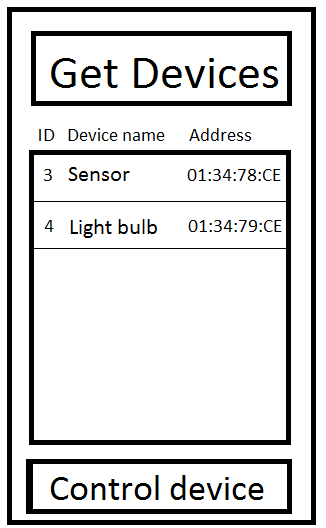
\includegraphics[width=0.4\textwidth]{pic1.png}
    \caption{The layout of the My Devices View}
    \label{fig:mydeviceview}
\end{figure}

\begin{figure}[H]
    \centering
    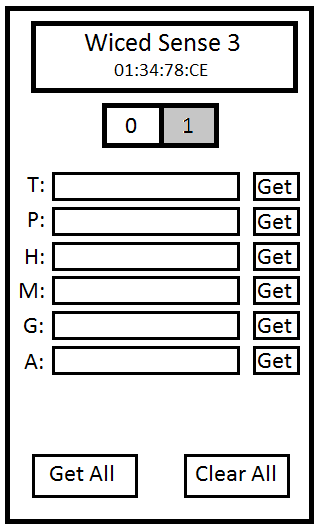
\includegraphics[width=0.4\textwidth]{pic2.png}
    \caption{The layout of the My Sensor View}
    \label{fig:mysensorview}
\end{figure}

\begin{figure}[H]
    \centering
    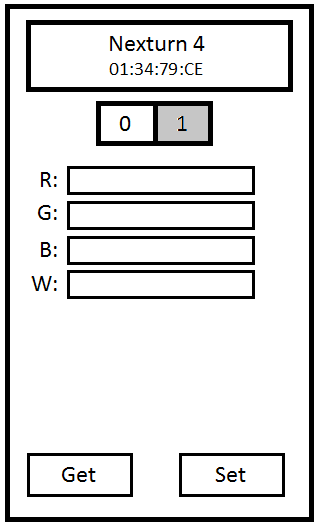
\includegraphics[width=0.3\textwidth]{pic3.png}
    \caption{The layout of the Light Bulb View}
    \label{fig:mylightbulbview}
\end{figure}

\end{description}
\end{document}
